% Sections/03_eda.tex
% Exploratory Data Analysis Section

\section{Exploratory Data Analysis}
\label{sec:eda}

We perform a range of analytics to understand the structure and relations within the UCI HAR dataset.

\subsection{Feature Value Distribution}
\label{subsec:feature_dist}

Box plots for all 50th features (representative sample out of all 561 features) indicate that values are successfully normalized to the range [-1.00, 1.00]. The majority of features have a median of 0 and an interquartile range of about 0.6, reflecting balanced spread of values. Outliers (points outside 1.5$\times$ interquartile range) are apparent for only a few features, reflecting some variation in movement measurements—which is inherent in human activity data.

\begin{figure}[htbp]
  \centering
  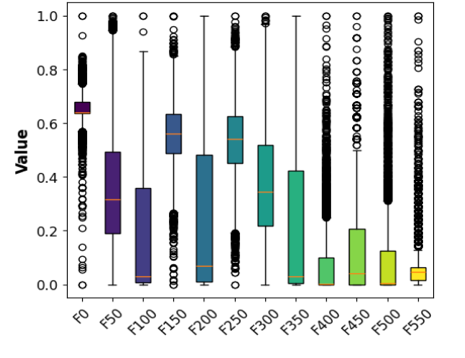
\includegraphics[width=0.7\textwidth]{figures/fig3.png}
  \caption{Plot shows the visual analysis of every 50th feature with the median and outliers of each of them}
  \label{fig:feature_dist_plot}
\end{figure}

\subsection{Feature Correlation Matrix}
\label{subsec:correlation}

Computing the Pearson correlation matrix for the first 30 features reveals a clear pattern of relationships:

\begin{itemize}
  \item Strong positive correlations ($r > 0.75$; deep red) are observed between features of correlated physical quantities on different sensor axes.
  \item Strong negative correlations ($r < -0.75$; dark blue) represent features that change in opposite directions, consistent with multi-axis sensor behavior.
  \item Approximately 20\% of feature pairs exhibit moderate-to-strong correlation ($|r| > 0.5$), uncovering strong redundancy.
  \item Less than 10\% of pairs demonstrate close-to-zero correlation (white/dim), validating that raw sensor signals strongly interrelate.
\end{itemize}

\begin{figure}[htbp]
  \centering
  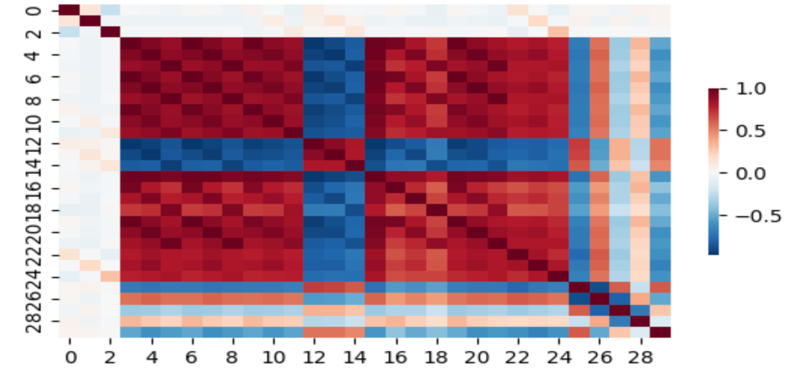
\includegraphics[width=0.7\textwidth]{figures/fig4.png}
  \caption{Correlation matrix visualizing positive (red) and negative (blue) feature relations}
  \label{fig:correlation_matrix}
\end{figure}

\subsection{Distribution Pattern Insights}
\label{subsec:insights}

These trends validate that normalization effectively normalizes sensor feature scales with significant redundancy, where features are essentially duplicates or well-predictable by others. This redundancy can be managed through dimensionality reduction (e.g., PCA) or more aggressive regularization, resulting in less overfitting, better interpretability, and more well-informed modeling choices for the pipeline.
